%%%%%%%%%%%%%%%%%%%%%%%%%%%%%%%%%%%%%%%%%
% Programming/Coding Assignment
% LaTeX Template
%
% This template has been downloaded from:
% http://www.latextemplates.com
%
% Original author:
% Ted Pavlic (http://www.tedpavlic.com)
%
% Note:
% The \lipsum[#] commands throughout this template generate dummy text
% to fill the template out. These commands should all be removed when 
% writing assignment content.
%
% This template uses a Perl script as an example snippet of code, most other
% languages are also usable. Configure them in the "CODE INCLUSION 
% CONFIGURATION" section.
%
%%%%%%%%%%%%%%%%%%%%%%%%%%%%%%%%%%%%%%%%%

%----------------------------------------------------------------------------------------
%	PACKAGES AND OTHER DOCUMENT CONFIGURATIONS
%----------------------------------------------------------------------------------------

\documentclass{article}

\usepackage{fancyhdr} % Required for custom headers
\usepackage{lastpage} % Required to determine the last page for the footer
\usepackage{extramarks} % Required for headers and footers
\usepackage[usenames,dvipsnames]{color} % Required for custom colors
\usepackage{graphicx} % Required to insert images
\usepackage{listings} % Required for insertion of code
\usepackage{courier} % Required for the courier font
\usepackage{lipsum} % Used for inserting dummy 'Lorem ipsum' text into the template
\usepackage{setspace}
\usepackage{color}
\usepackage{comment}
\usepackage{caption}

\usepackage{hyperref}
\usepackage{natbib}
\usepackage{underscore}
\usepackage{subfigure}
\usepackage{fixltx2e}

\hypersetup{
    colorlinks=true,
    linkcolor=blue,
    filecolor=magenta,      
    urlcolor=cyan,
    breaklinks=true
}

%\usepackage[]{algorithm2e}
\usepackage{pdfpages}




%For python inclusion (http://widerin.org/blog/syntax-highlighting-for-python-scripts-in-latex-documents)
\definecolor{Code}{rgb}{0,0,0}
\definecolor{Decorators}{rgb}{0.5,0.5,0.5}
\definecolor{Numbers}{rgb}{0.5,0,0}
\definecolor{MatchingBrackets}{rgb}{0.25,0.5,0.5}
\definecolor{Keywords}{rgb}{0,0,1}
\definecolor{self}{rgb}{0,0,0}
\definecolor{Strings}{rgb}{0,0.63,0}
\definecolor{Comments}{rgb}{0,0.63,1}
\definecolor{Backquotes}{rgb}{0,0,0}
\definecolor{Classname}{rgb}{0,0,0}
\definecolor{FunctionName}{rgb}{0,0,0}
\definecolor{Operators}{rgb}{0,0,0}
\definecolor{Background}{rgb}{0.98,0.98,0.98}

% Margins
\topmargin=-0.45in
\evensidemargin=0in
\oddsidemargin=0in
\textwidth=6.5in
\textheight=9.0in
\headsep=0.25in

\linespread{1.1} % Line spacing

% Set up the header and footer
\pagestyle{fancy}
\lhead{\hmwkAuthorName} % Top left header
%\chead{\hmwkClass\ (\hmwkClassInstructor\ \hmwkClassTime): \hmwkTitle} % Top center head
\chead{\hmwkClass\ (\hmwkClassInstructor): \hmwkTitle} % Top center head
\rhead{\firstxmark} % Top right header
\lfoot{\lastxmark} % Bottom left footer
\cfoot{} % Bottom center footer
\rfoot{Page\ \thepage\ of\ \protect\pageref{LastPage}} % Bottom right footer
\renewcommand\headrulewidth{0.4pt} % Size of the header rule
\renewcommand\footrulewidth{0.4pt} % Size of the footer rule

\setlength\parindent{0pt} % Removes all indentation from paragraphs

%----------------------------------------------------------------------------------------
%	CODE INCLUSION CONFIGURATION
%----------------------------------------------------------------------------------------

\definecolor{MyDarkGreen}{rgb}{0.0,0.4,0.0} % This is the color used for comments
\lstloadlanguages{Perl} % Load Perl syntax for listings, for a list of other languages supported see: ftp://ftp.tex.ac.uk/tex-archive/macros/latex/contrib/listings/listings.pdf
\lstset{language=Perl, % Use Perl in this example
        frame=single, % Single frame around code
        basicstyle=\small\ttfamily, % Use small true type font
        keywordstyle=[1]\color{Blue}\bf, % Perl functions bold and blue
        keywordstyle=[2]\color{Purple}, % Perl function arguments purple
        keywordstyle=[3]\color{Blue}\underbar, % Custom functions underlined and blue
        identifierstyle=, % Nothing special about identifiers                                         
        commentstyle=\usefont{T1}{pcr}{m}{sl}\color{MyDarkGreen}\small, % Comments small dark green courier font
        stringstyle=\color{Purple}, % Strings are purple
        showstringspaces=false, % Don't put marks in string spaces
        tabsize=5, % 5 spaces per tab
        %
        % Put standard Perl functions not included in the default language here
        morekeywords={rand},
        %
        % Put Perl function parameters here
        morekeywords=[2]{on, off, interp},
        %
        % Put user defined functions here
        morekeywords=[3]{test},
       	%
        morecomment=[l][\color{Blue}]{...}, % Line continuation (...) like blue comment
        numbers=left, % Line numbers on left
        firstnumber=1, % Line numbers start with line 1
        numberstyle=\tiny\color{Blue}, % Line numbers are blue and small
        stepnumber=5 % Line numbers go in steps of 5
}

% Creates a new command to include a perl script, the first parameter is the filename of the script (without .pl), the second parameter is the caption
\newcommand{\perlscript}[2]{
\begin{itemize}
\item[]\lstinputlisting[caption=#2,label=#1]{#1.pl}
\end{itemize}
}


%----------------------------------------------------------------------------------------
%	DOCUMENT STRUCTURE COMMANDS
%	Skip this unless you know what you're doing
%----------------------------------------------------------------------------------------

% Header and footer for when a page split occurs within a problem environment
\newcommand{\enterProblemHeader}[1]{
\nobreak\extramarks{#1}{#1 continued on next page\ldots}\nobreak
\nobreak\extramarks{#1 (continued)}{#1 continued on next page\ldots}\nobreak
}

% Header and footer for when a page split occurs between problem environments
\newcommand{\exitProblemHeader}[1]{
\nobreak\extramarks{#1 (continued)}{#1 continued on next page\ldots}\nobreak
\nobreak\extramarks{#1}{}\nobreak
}

\setcounter{secnumdepth}{0} % Removes default section numbers
\newcounter{homeworkProblemCounter} % Creates a counter to keep track of the number of problems

\newcommand{\homeworkProblemName}{}
\newenvironment{homeworkProblem}[1][Problem \arabic{homeworkProblemCounter}]{ % Makes a new environment called homeworkProblem which takes 1 argument (custom name) but the default is "Problem #"
\stepcounter{homeworkProblemCounter} % Increase counter for number of problems
\renewcommand{\homeworkProblemName}{#1} % Assign \homeworkProblemName the name of the problem
\section{\homeworkProblemName} % Make a section in the document with the custom problem count
\enterProblemHeader{\homeworkProblemName} % Header and footer within the environment
}{
\exitProblemHeader{\homeworkProblemName} % Header and footer after the environment
}

\newcommand{\problemAnswer}[1]{ % Defines the problem answer command with the content as the only argument
\noindent\framebox[\columnwidth][c]{\begin{minipage}{0.98\columnwidth}#1\end{minipage}} % Makes the box around the problem answer and puts the content inside
}

\newcommand{\homeworkSectionName}{}
\newenvironment{homeworkSection}[1]{ % New environment for sections within homework problems, takes 1 argument - the name of the section
\renewcommand{\homeworkSectionName}{#1} % Assign \homeworkSectionName to the name of the section from the environment argument
\subsection{\homeworkSectionName} % Make a subsection with the custom name of the subsection
\enterProblemHeader{\homeworkProblemName\ [\homeworkSectionName]} % Header and footer within the environment
}{
\enterProblemHeader{\homeworkProblemName} % Header and footer after the environment
}

%----------------------------------------------------------------------------------------
%	NAME AND CLASS SECTION
%----------------------------------------------------------------------------------------

\newcommand{\hmwkTitle}{Assignment\ \#1 } % Assignment title
%\newcommand{\hmwkDueDate}{Monday,\ January\ 1,\ 2012} % Due date
\newcommand{\hmwkClass}{Introduction to Digital Libraries} % Course/class
%\newcommand{\hmwkClassTime}{10:30am} % Class/lecture time
\newcommand{\hmwkClassInstructor}{Dr. Nelson} % Teacher/lecturer
\newcommand{\hmwkAuthorName}{Alexander Nwala} % Your name

%----------------------------------------------------------------------------------------
%	TITLE PAGE
%----------------------------------------------------------------------------------------

\title{
\vspace{2in}
\textmd{\textbf{\hmwkClass:\ \hmwkTitle}}\\
%\normalsize\vspace{0.1in}\small{Due\ on\ \hmwkDueDate}\\
%\vspace{0.1in}\large{\textit{\hmwkClassInstructor\ \hmwkClassTime}}
\vspace{0.1in}\large{\textit{\hmwkClassInstructor}}
\vspace{3in}
}

\author{\textbf{\hmwkAuthorName}}
\date{Thursday, February 12, 2015} % Insert date here if you want it to appear below your name

%----------------------------------------------------------------------------------------

\begin{document}

\maketitle



%----------------------------------------------------------------------------------------
%	TABLE OF CONTENTS
%----------------------------------------------------------------------------------------

%\setcounter{tocdepth}{1} % Uncomment this line if you don't want subsections listed in the ToC

\newpage
\tableofcontents
\newpage

%----------------------------------------------------------------------------------------
%	PROBLEM 1
%----------------------------------------------------------------------------------------

% To have just one problem per page, simply put a \clearpage after each problem

\begin{homeworkProblem}

Write a program that extracts 10000 tweets with links from Twitter. 
Reference: \url{http://thomassileo.com/blog/2013/01/25/using-twitter-rest-api-v1-dot-1-with-python/}. Other similar resources are available.\\
Note that only Twitter API 1.1 is currently available; version 1 code will no longer work.\\


Save the tweet URIs, and the mapping to the link(s) each tweet contains
Note: tweets can have \textgreater 1 links\\
For each t.co link, use \begin{verbatim}    "curl -I -L"\end{verbatim} to record the HTTP headers all the way to a terminal HTTP status (i.e. chase down all the redirects)\\

How many unique final URIs? How many duplicate URIs?
Build a histogram of how many redirects (every URI will have at least 1)
\url{http://en.wikipedia.org/wiki/Histogram}
Build a histogram of HTTP status codes encountered (you'll have at least 20000: 10000 301s, and 10000+ more)


%\problemAnswer
%{
    \begin{verbatim}\end{verbatim}
    \textbf{SOLUTION}\\


    The solution for this problem is outlined by the following steps:
    \begin{enumerate}

    \item \textbf{Extract Tweets:} This was achieved by utilizing Tweepy's \cite{Tweepy} Twitter search API. As outlined by Listing 1. the tweets were extracted using the query:

    \begin{verbatim}
        http://www.
    \end{verbatim}

    To extract 30 tweets which fulfill the search criteria. However, in order not to exceed Twitter's rate limiting on search \cite{TwitterRateLimit}, Listing 1. sleeps in between requests. 

    \lstinputlisting[breaklines=true, caption=Extract Tweets]{extractTweetsSnippet.py}

    \item \textbf{Follow redirects, count redirects, and record HTTP status codes:} Given that Twitter shortens URIs embedded in Tweets, Listing 2. resolves redirections by continuously retrieving the URIs in the Location attribute of the 301 responses. This is done until the final URI is retrieved. Listing 2. also counts the number of redirections and stores the HTTP status codes simultaneously.

    \lstinputlisting[breaklines=true, caption=Extract Tweets]{redirectOperationsSnippet.py}

    \begin{verbatim}
    The file originalLinksFile.txt contains the complete data of form: 
    
    <
    TWEET ID: Unique Identifier for a Tweets
    URI: Final URI derived by following the redirects
    REDIRECTION COUNT: The number of redirections
    [REDIRECTION CODES]: A list of HTTP response status codes seen while 
    following redirects
    TWEET CREATED AT DATETIME: The timestamp on Tweets
    >
    \end{verbatim}

    \item \textbf{Count unique URIs:} Based on Listing 3. This statistic was collected: out of 10,000 Tweets collected, 9,442 tweets were unique, however, only 2,165 URIs were unique. This was due to overlapping search results.

    \lstinputlisting[breaklines=true, caption=Count Unique URIs]{countUniqueURIsSnippet.py}

    \item \textbf{Draw histograms:} Due to Listing 4. Chart 1. summarizes the distribution of HTTP status codes. and Chart 2. summarizes the distribution of redirection counts.

    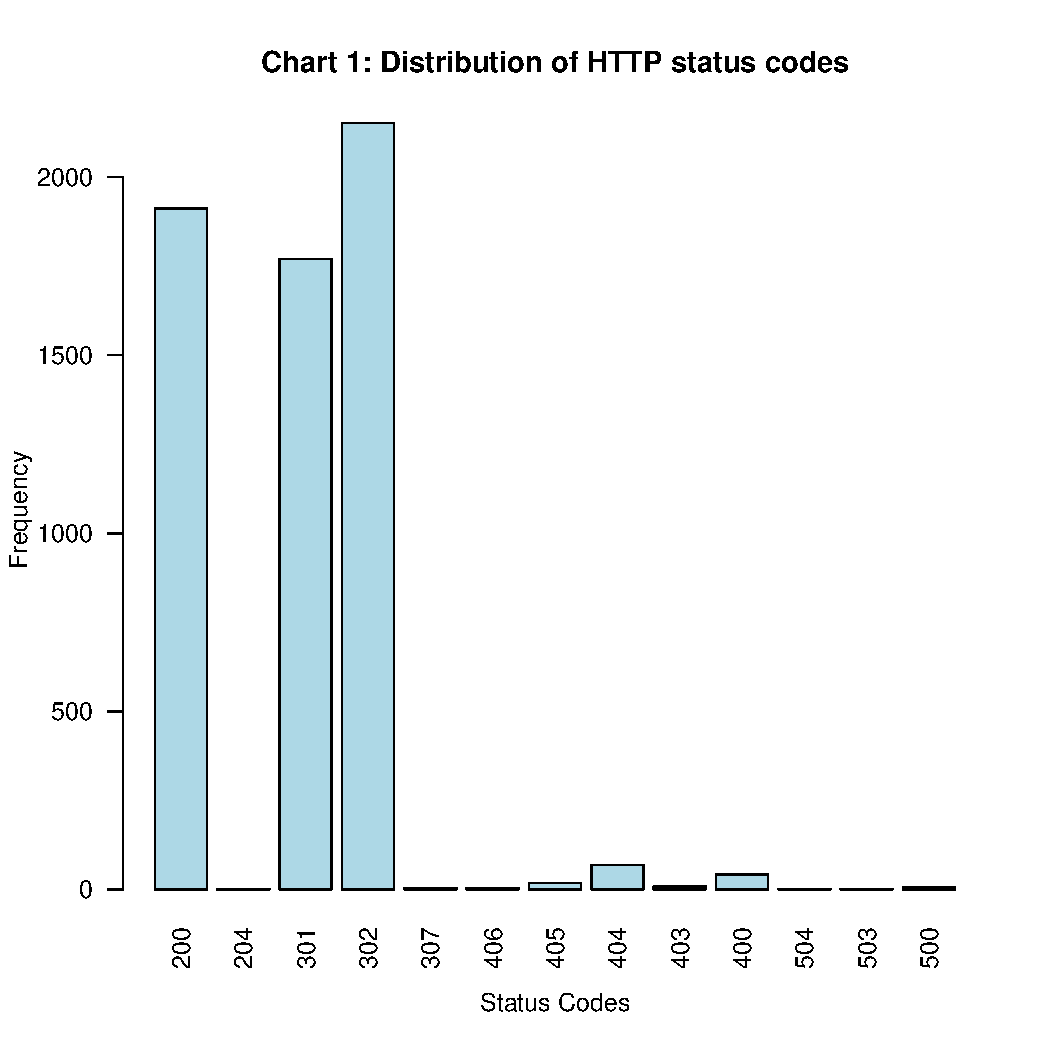
\includepdf[width=\textwidth, pages={1}]{../Rplots.pdf}
    \includepdf[width=\textwidth, pages={2}]{../Rplots.pdf}


    \lstinputlisting[breaklines=true, caption=Draw Histograms]{/home/anwala/CS851/Assignment1/histogramAndGraph.r}

    \begin{verbatim}
    The file unique_originalLinksFile.txt contains data in the same format 
    as originalLinksFile.txt, but does not contain duplicates
    \end{verbatim}


    
    \end{enumerate}
   

%}

\end{homeworkProblem}

%----------------------------------------------------------------------------------------
%   PROBLEM 2
%----------------------------------------------------------------------------------------

\begin{homeworkProblem}

Use ``Carbon Date'' to estimate the age of each link(s) in a tweet
See: \url{http://ws-dl.blogspot.com/2013/04/2013-04-19-carbon-dating-web.html}\\
Create a histogram of ( Age\textsubscript{tweet} - Age\textsubscript{link} )
Many (most?) deltas will be 0, but there should be many \textgreater  0
For these deltas, compute: median, mean, std dev, std err.
Use wget to download the text for all the links.  Hold on to those, we’ll come back to them later. See:\\

http://superuser.com/questions/55040/save-a-single-web-page-with-background-images-with-wget\\
http://stackoverflow.com/questions/6348289/download-a-working-local-copy-of-a-webpage


%\problemAnswer
%{
    \begin{verbatim}\end{verbatim}
    \textbf{SOLUTION}\\


    The solution for this problem is outlined by the following steps:
    \begin{enumerate}

    \item \textbf{Carbon date URIs:} This was achieved by \url{https://github.com/HanySalahEldeen/CarbonDate} The estimated creation date of the URIs from \textbf{unique_originalLinksFile.txt} was written into \textbf{final_cd_unique_unique_originalLinksFile.txt}. Below is a summary are the summary statistics derived (Listing 4.) from the the difference between the Tweets age and the estimated creation date from Carbon Date for 1,684 URIs. 

    \begin{verbatim}
        Mean: 774.7267 days
        Median: 58 days
        Standard Deviation: 1250.453
        Standard Error: 30.48073
    \end{verbatim}

    Based on the foregoing data, it can be seen that the age values is highly skewed to the left (Approaching 0), probably because the links in many Tweets are new, hence unlikely to have been archived.

    \item \textbf{Draw histogram:} Chart 3. due to Listing 4. outlines a histogram of Age\textsubscript{tweet} - Age\textsubscript{link} entries from \textbf{DELTA_DAYS.txt} derived from \textbf{final_cd_unique_unique_originalLinksFile.txt}

    \includepdf[width=\textwidth, pages={3}]{../Rplots.pdf}

    \item \textbf{Download HTML text of links:} Based on input from \textbf{unique_originalLinksFile.txt}, Listing 5. utilizes curl to download and save the HTML text of the links into the folder RawHtml, the file names were derived from a hash calculated from the respective URIs.

    \lstinputlisting[breaklines=true, caption=Download HTML]{extractHTMLSnippet.py}

    \end{enumerate}
   

%}

\end{homeworkProblem}
\bibliographystyle{plain}
\bibliography{A1bibFile}

\end{document}